\chapter{Deterministic Optimization Across Worlds}
\label{chapter-18-deterministic-optimization-across-worlds}

\begin{quote}
\emph{Navigating the Rulial Manifold to discover structurally superior universes.}
\end{quote}

For decades, software optimization has been treated as a dark art. It exists as a collection of tribal knowledge, a bag of disconnected heuristics, and a series of aggressive compiler passes that hope for the best. Engineers tweak flags, unroll loops manually, and pray that the black box of the compiler understands their intent. It is a frantic search through a disorganized state space, governed by luck as much as logic.

However, once we accept the premise that computation is geometry, this chaotic approach becomes obsolete. Optimization transforms from an act of guesswork into an act of navigation. We are no longer merely ``improving code'' or shuffling instructions; we are selecting superior worldlines from the local Rulial manifold. We are not applying arbitrary transformation passes; we are steering the flow of computation toward geodesics—the mathematically shortest paths between intent and result.

In the \textbf{C$\Omega$MPUTER} paradigm, you are not guessing what the optimizer might do. You are choosing the shortest legal path through a structured, metric space of possibilities. This chapter details the transition from heuristic hope to deterministic, geometric traversal of nearby universes.

\section{Optimization as Worldline Navigation}
\label{optimization-as-worldline-navigation}

To understand optimization, we must first recognize that every execution trace—every worldline—is merely one path through the vast possibility space of the WARP Graph (WARP). Not all paths are created equal. Some worldlines are short, smooth, and stable; they respect invariants and minimize computational effort. Others are long, jagged, and fragile, meandering through high-entropy states and structural inefficiencies.

In the WARP+DPO (Double-Pushout) worldview, optimization is defined as steering the collapse of the bundle toward these cleaner, shorter paths. We do not mutate the code in the traditional sense; rather, we mutate the worldline by imparting intelligence to the collapse mechanism. By analyzing the geometry of Rulial Space, we can identify which branches of the Time Cone lead to efficient outcomes and which lead to redundant cycles. Optimization is the art of ensuring the system falls into the most efficient basin of attraction.

\begin{figure}[h]
\centering
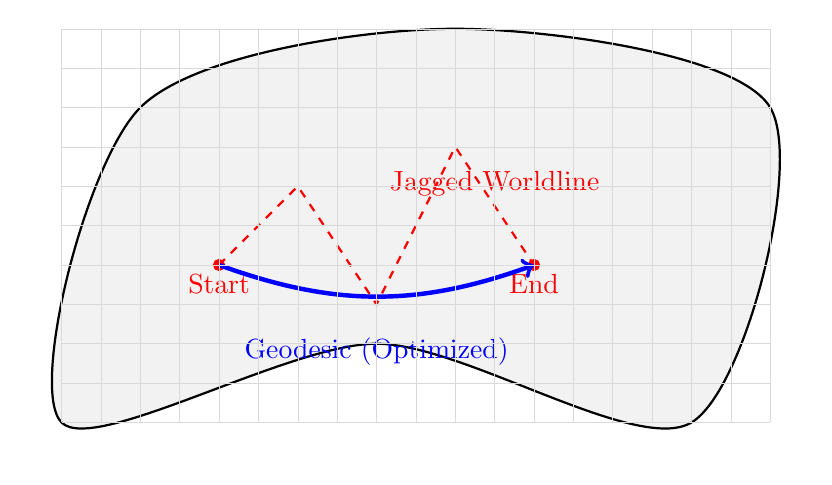
\begin{tikzpicture}
    % Draw the manifold surface
    \draw[thick, fill=gray!10] plot [smooth cycle] coordinates {(0,0) (4,1) (8,0) (9,4) (5,5) (1,4)};
    
    % Draw a "Jagged" unoptimized path
    \draw[red, thick, dashed] (2,2) -- (3,3) -- (4,1.5) -- (5,3.5) -- (6,2) node[midway, above] {Jagged Worldline};
    \filldraw[red] (2,2) circle (2pt) node[below] {Start};
    \filldraw[red] (6,2) circle (2pt) node[below] {End};

    % Draw a "Geodesic" optimized path
    \draw[blue, ultra thick, ->] (2,2) to[out=-20, in=200] (6,2);
    \node[blue, below] at (4,1.2) {Geodesic (Optimized)};

    % Grid lines for "geometry" feel
    \draw[step=0.5cm, gray!30, very thin] (0,0) grid (9,5);
\end{tikzpicture}
\caption{Optimization as Navigation: The naive execution (red) traverses a high-cost, jagged path. The optimized execution (blue) follows the geodesic—the smoothest path allowed by the manifold's curvature.}
\end{figure}

\section{The Optimizer's Input: The Bundle at Each Tick}
\label{the-optimizers-input-the-bundle-at-each-tick}

The fundamental unit of operation for the optimizer is the rewrite bundle. At every single tick of the clock, the current universe presents a bundle of all legal rewrites available to the Scheduler. This is the raw material of the future.

Each candidate rewrite is not just a syntactic tweak. It carries a small packet of geometric and resource data:

\begin{itemize}
  \item how it changes Rulial Distance (structural effort),
  \item how it bends or flattens local curvature,
  \item how it interferes or composes with other rules,
  \item how it moves the system along concrete resource axes: time, memory, bandwidth, energy, risk.
\end{itemize}

The optimizer functions as a geometric filter. It examines every potential rewrite in the bundle and evaluates them against rigorous criteria. It asks which rewrite most effectively shortens the global path to the objective \emph{under the current cost model}. It analyzes which rewrite reduces the local curvature, making the system more stable. It determines which rewrite best preserves critical invariants and which maximizes the width of future bundles, thereby preserving optionality. Crucially, it identifies which rewrites move the system closer to a known geodesic and which risk bending the worldline into pathological regions of high friction.

Formally, each rewrite $r$ at state $s$ is annotated with a resource vector and evaluated by a \emph{Lagrangian of Computation} (Section~\ref{lagrangian-of-computation}), which collapses ``CPU vs memory vs bandwidth vs risk'' into a single scalar cost. The optimizer never asks ``Is this rewrite good in general?'' It asks the only question that matters: \emph{Does this rewrite move us downhill in this universe, under these constraints, right now?}

This process replaces the ``optimization passes'' of traditional compilers. Instead of applying a fixed sequence of transformations, the system makes dynamic, context-aware choices based on the computable gradient of the state space.

\section{Local Optimization: Following the Gradient of the Manifold}
\label{local-optimization-following-the-gradient-of-the-manifold}

Every legal rewrite carries specific geometric data: a local resource vector, an induced scalar cost from the Lagrangian, a structural effect on the graph (curvature), and an interference pattern with other rules. By aggregating these factors, the optimizer can compute a local gradient in Rulial Space. This vector points in the direction of steepest descent toward a simpler, lower-energy universe, as measured by your chosen cost function.

This mechanism is the computational equivalent of gradient descent, hill-climbing, or Newton's method, but it operates on the topology of the WARP graph rather than on numerical landscapes. The system essentially ``rolls downhill,'' following the natural contours of the rule set toward a state of minimal cost. Where traditional optimization frameworks hand-wave about `hot paths' and `critical sections,' the WARP-based optimizer computes an explicit, discrete Rulial gradient and walks it.

\begin{figure}[h]
\centering
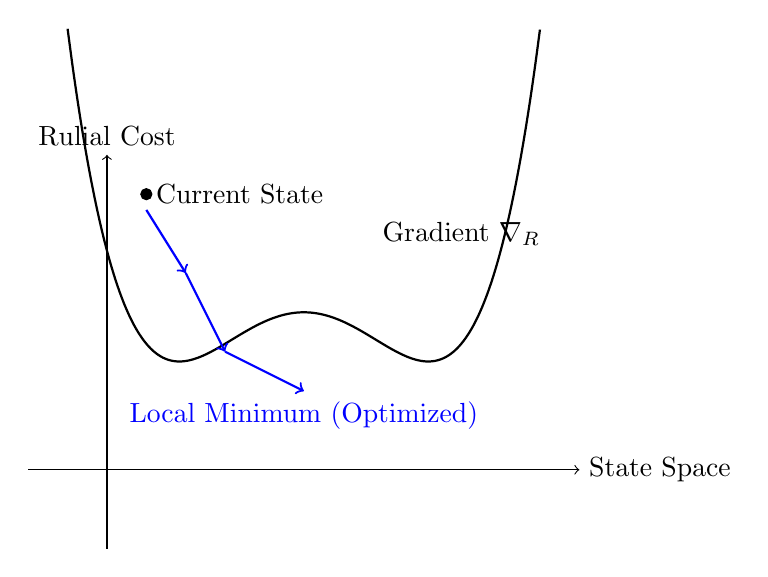
\begin{tikzpicture}
    % Axes
    \draw[->] (-1,0) -- (6,0) node[right] {State Space};
    \draw[->] (0,-1) -- (0,4) node[above] {Rulial Cost};

    % Potential Well Function
    \draw[thick, domain=-0.5:5.5, smooth, samples=100] plot (\x, {0.1*(\x-2.5)^4 - 0.5*(\x-2.5)^2 + 2});

    % Current State
    \filldraw[black] (0.5, 3.5) circle (2pt) node[right] {Current State};
    
    % Gradient Arrows
    \draw[->, thick, blue] (0.5, 3.3) -- (1.0, 2.5);
    \draw[->, thick, blue] (1.0, 2.5) -- (1.5, 1.5);
    \draw[->, thick, blue] (1.5, 1.5) -- (2.5, 1.0) node[below] {Local Minimum (Optimized)};

    % Annotations
    \node at (4.5, 3) {Gradient $\nabla_{R}$};
\end{tikzpicture}
\caption{Local Optimization: The optimizer calculates the Rulial Gradient ($\nabla_{R}$) at the current state and selects the rewrite that descends the cost surface most rapidly.}
\end{figure}

\section{Global Optimization: Finding Geodesics}
\label{global-optimization-finding-geodesics}

While local optimization handles immediate efficiency, global optimization seeks the geodesic: the lowest-cost legal worldline between the start state and the target state, measured under the Lagrangian of Computation. Traditional compilers attempt to approximate this using layers of brittle heuristics. In the \textbf{C$\Omega$MPUTER} framework, we find geodesics by combining structured search across counterfactual universes with rigorous curvature analysis.

By analyzing the interference patterns (Chapter 12) and Rulial metrics (Chapter 5), the system can look ahead. It creates a map of the future cone, identifying paths that may initially look expensive but eventually open up ``wormholes''—shortcuts through the state space that bypass vast amounts of computation. Some worldlines take a few costly steps to align themselves with a low-curvature corridor and then run almost frictionlessly. Others save a tiny amount now and spend massively later.

Global optimization is the art of paying a little to get into the right corridor. The search operates over bundles and counterfactual futures, but it is always constrained by legality and invariants. We are not inventing new mathematics in the dark; we are surfacing the shortest lawful path that already exists inside the rule system.

\section{Counterfactual Optimization: The Synthesis}
\label{counterfactual-optimization-cfee-optimizer-magic}

The true power of this architecture emerges when we combine the Counterfactual Execution Engine (CFEE) from Chapter 16 with the optimizer. This combination yields Deterministic Multiverse Optimization.

In this cycle, the CFEE proposes alternative futures by spawning parallel universes. The optimizer then evaluates these futures using the Lagrangian-based geometric metrics. Finally, the Scheduler collapses reality onto the best performing branch. The system essentially ``peeks'' into nearby universes to see which timeline offers the flattest curvature and the most direct path to the target. It dismisses brittle or high-cost alternatives before they become reality. It is a form of look-ahead that feels prescient, but is grounded entirely in the deterministic geometry of the bundle.

\begin{figure}[h]
\centering
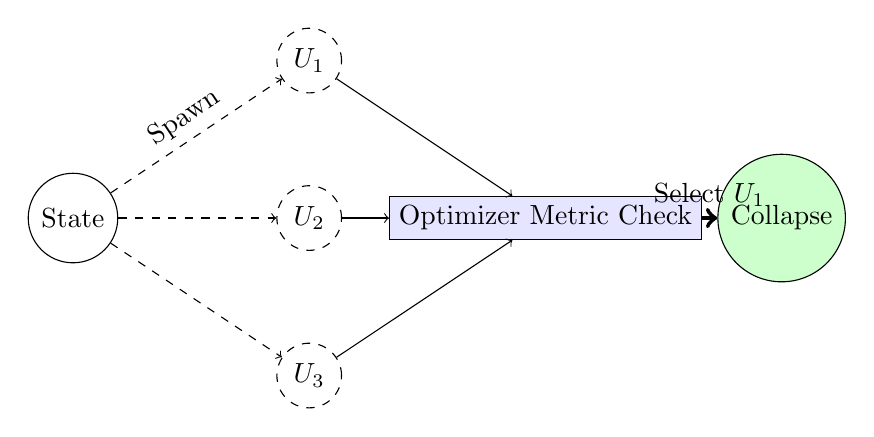
\begin{tikzpicture}
    % Central Node
    \node[circle, draw, minimum size=1cm] (Start) at (0,0) {State};

    % Counterfactual Branches
    \node[circle, draw, dashed, minimum size=0.8cm] (CF1) at (3, 2) {$U_1$};
    \node[circle, draw, dashed, minimum size=0.8cm] (CF2) at (3, 0) {$U_2$};
    \node[circle, draw, dashed, minimum size=0.8cm] (CF3) at (3, -2) {$U_3$};

    % Edges representing CFEE spawn
    \draw[->, dashed] (Start) -- (CF1) node[midway, above, sloped] {Spawn};
    \draw[->, dashed] (Start) -- (CF2);
    \draw[->, dashed] (Start) -- (CF3);

    % Optimizer Selection
    \node[rectangle, draw, fill=blue!10] (Opt) at (6, 0) {Optimizer Metric Check};
    \draw[->] (CF1) -- (Opt);
    \draw[->] (CF2) -- (Opt);
    \draw[->] (CF3) -- (Opt);

    % Collapse
    \node[circle, draw, fill=green!20, minimum size=1cm] (End) at (9, 0) {Collapse};
    \draw[->, ultra thick] (Opt) -- (End) node[midway, above] {Select $U_1$};

\end{tikzpicture}
\caption{The Optimization Cycle: The CFEE spawns candidate universes ($U_1, U_2, U_3$). The Optimizer measures their geometric cost under the Lagrangian. The Scheduler collapses reality into the optimal path ($U_1$).}
\end{figure}

\section{Optimization as Rulial Shaping}
\label{optimization-as-rulial-shaping}

Optimizing code in the WARP+DPO worldview is best understood as shaping the system's possibility geometry so that favorable futures become inevitable and pathological futures become topologically impossible.

This is distinct from the manual application of transformations or the micromanagement of instruction ordering. Instead, it involves designing robust invariants and choosing rules that reinforce smoothness. It requires strengthening K-interfaces to forbid illegal states and introducing canonical forms that reduce the search space. By reducing destructive interference and increasing constructive interference, we flatten curvature spikes and straighten the worldlines. We are, in effect, engineering smooth universes where the ``path of least resistance'' happens to be the correct one.

There are two levers here:

\begin{itemize}
  \item \textbf{Hard geometry} — the rule set and invariants, which define what is legal and how bundles branch.
  \item \textbf{Soft geometry} — the Lagrangian of Computation, which says which legal directions are cheap vs expensive.
\end{itemize}

Changing the rules reshapes the manifold itself. Changing the Lagrangian leaves the manifold intact but tilts the gradient field that flows across it. Together, they let you sculpt a universe where the optimizer does not fight the physics of your system—it rides it.

\section{The Fundamental Metric: Rulial Distance}
\label{rulial-distance-as-an-optimization-cost-function}

\noindent\textbf{Note.} The Rulial Distance used in this chapter is the weighted generalization of the distance introduced in Chapter~5. There, each rewrite had unit cost; here, the Lagrangian $\mathcal{L}(r,s)$ assigns a resource-aware cost, and $d_{\mathcal{R}}$ is defined as the infimum of total Lagrangian action across all worldlines.

The central innovation here is the replacement of heuristic guesswork with a concrete metric. The optimizer functions by minimizing the Rulial Distance between the current state and the target state—but now understood through the lens of a cost-weighted worldline.

As defined in Chapter 5, Rulial Distance $d(s,t)$ is the minimal number of legal rewrites required to transform one frozen computation into another. It is a directed pseudometric on the Rulial state space: it tells you \emph{how many} steps separate two worlds, not yet how much those steps ``hurt.''

Rulial Distance is computable, structural, geometric, and rule-sensitive. It honors invariants and provides the bare, structural notion of effort. This replaces the black-box intuition of traditional compiler optimizations with an explicit, quantifiable substrate.

On top of this substrate, the Lagrangian of Computation assigns a cost to each step. The distance between two worlds, from the optimizer's point of view, is no longer just ``how many rewrites'' but ``what is the minimum Lagrangian cost over all legal rewrite paths between them.'' We move from hoping a heuristic works to:

\begin{enumerate}
  \item measuring structural distance in Rulial Space, and
  \item minimizing a clear, resource-aware cost functional over that space.
\end{enumerate}

This fundamentally alters the reliability and transparency of the optimization process. When something is ``faster'' or ``cheaper,'' we can say exactly in which metric, by how much, and along which geodesic.

\section{The Lagrangian of Computation: What ``Cost'' Actually Means}
\label{lagrangian-of-computation}

Rulial Distance tells you how many legal rewrites separate two states. Real machines care about more than just how many steps they take.

A rewrite can be cheap in time but expensive in memory, or vice versa. Some steps are almost free until you cross a cache boundary or saturate a network link. Others introduce numerical risk, privacy risk, or external costs (like re-running a third-party service). If we pretend all steps cost the same, we get pretty geometry and terrible systems.

To make optimization honest, we attach a local resource vector to every rewrite:
\[
\rho(r, s) = (\Delta T, \Delta M, \Delta B, \Delta E, \Delta R, \dots)
\]
capturing the change in time, memory, bandwidth, energy, risk, and whatever else you care about when applying rewrite $r$ at state $s$.

The optimizer does not juggle a dozen objectives independently. It pushes them through a single scalar cost functional, the \emph{Lagrangian of Computation}:
\[
\mathcal{L}(r, s) \;=\; w_T \cdot \Delta T
  \;+\; w_M \cdot \Delta M
  \;+\; w_B \cdot \Delta B
  \;+\; w_E \cdot \Delta E
  \;+\; w_R \cdot \Delta R
  \;+\; \dots
\]

The weights $w_\bullet$ are not universal constants. They encode your constraints:

\begin{itemize}
  \item On a phone, energy and memory get heavy weights; latency gets a softer one.
  \item In low-latency trading, wall-clock time dominates; memory is almost free.
  \item In a regulated environment, ``risk'' (breaking an invariant, violating a policy) is effectively infinite.
\end{itemize}

A worldline
\[
\gamma = (s_0 \to s_1 \to \dots \to s_k)
\]
then has total cost
\[
C(\gamma) = \sum_{i=0}^{k-1} \mathcal{L}(r_i, s_i),
\]
where each $r_i$ is the rewrite used from $s_i$ to $s_{i+1}$.

Geodesic search is now well-defined: among all legal worldlines from the start to the target, we choose the one minimizing $C(\gamma)$. Rulial Distance still measures the structural effort in terms of rewrites; the Lagrangian tells us which effort actually matters.

Changing the weights does not change which states are reachable. It changes which directions look ``downhill.'' Tuning the Lagrangian literally bends the optimization geometry around your business constraints. When you say ``we care more about memory than CPU cycles,'' you are not making a vague product statement—you are redefining the metric tensor of your computational universe.

\section{Low Curvature Equals Better Optimization}
\label{low-curvature-better-optimization}

There is a direct correlation between the curvature of the manifold and the efficacy of optimization. In regions of low curvature, bundles align, worlds remain structurally similar, and collapse is stable. Optimization feels natural because the gradient is smooth; geodesics are easy to locate and CFEE branches quickly converge on similar low-cost futures.

Conversely, high curvature introduces conflict. Bundles interfere destructively, worlds diverge rapidly, and collapse becomes unstable. In these regions, optimization feels impossible because the geometry itself fights against linearization; tiny local choices induce massive global differences. You can still search, but the gradient keeps lying to you.

Crucially, curvature is not an abstract aesthetic property; it is measured with respect to your cost model. Weight memory more heavily, and directions that allocate memory become ``steeper.'' Weight latency more heavily, and long sequential chains become cliffs. The same rule system can present low curvature to one Lagrangian and brutal curvature to another.

This provides a crucial structural insight for system designers: if you desire highly optimized systems, you must design low-curvature rule sets \emph{relative to the cost model you actually care about}. This vocabulary allows us to articulate architectural flaws that were previously invisible: ``This API is not slow because the compiler is dumb. It is slow because the rule geometry around it is high-curvature with respect to latency.''

\section{The Horizon of Optimizability}
\label{horizon-of-optimizability}

Optimization is not infinite. For any fixed rule set and cost model, there is a point beyond which the geometry stops helping you.

In some regions of Rulial Space, the bundles are structured: some edges are much cheaper than others; the gradient clearly points ``downhill.'' In other regions, every legal rewrite has roughly the same Lagrangian cost. The bundles are almost isotropic, interference is violent, and nearby worlds look like unstructured noise. In those zones, there is no cheap direction left. The only way forward is to pay full price.

We call the boundary between these regimes the \emph{Horizon of Optimizability}.

Informally: starting from a state $s$, you can optimize within the horizon—shortening worldlines, flattening curvature, finding wormholes. Beyond the horizon, any further savings would require changing the rule system or breaking invariants. You can move, but you cannot move \emph{more cheaply} without changing the laws of your universe.

This shows up everywhere:

\begin{itemize}
  \item Cryptographic hashes are deliberately engineered to sit beyond the horizon. Each step scrambles structure so thoroughly that, under the cryptographic invariants, the cheapest way to ``compute the hash'' is to actually run the hash. Any geodesic that looks shorter is illegal.
  \item High-quality PRNGs, perfect shuffles, and some chaotic simulations intentionally erase exploitable local curvature. The manifold is still there, but all nearby directions cost the same. There is no gradient to follow without changing semantics.
\end{itemize}

From the optimizer’s point of view, a horizon is detectable. As it explores bundles and counterfactual futures, it can see when gradients flatten out, when candidate geodesics converge to the same total cost, and when CFEE branches fail to expose cheaper alternatives. At that point, it stops pretending: further local search is wasted unless you modify the rules themselves (the MR axis, Section~\ref{multi-model-optimization-mr-axis}) or relax your invariants.

This is a feature, not a failure. Good system design places security-critical or irreducible components \emph{beyond} the horizon, and keeps everything else in smooth, low-curvature regions where the optimizer can actually do work.

\section{Multi-Model Optimization: The MR Axis}
\label{multi-model-optimization-mr-axis}

Finally, we must consider the broader context of the Multi-Rule (MR) axis. Optimization is not strictly limited to choosing the best future within a fixed set of rules. It also involves choosing the best set of rules for the problem at hand.

By modifying K-interfaces, altering rewrite patterns, refining invariants, or adjusting recursion strategies, we can produce entirely new universes that inherently optimize better. This is Multi-Model (MRMW) optimization: the simultaneous optimization of the worldline within a universe and the optimization of the universe itself. This represents the pinnacle of structured computation—a system that can rewrite its own laws to better solve the problem it faces.

The Horizon of Optimizability makes MRMW optimization unavoidable. Once the optimizer detects that, under the current rules and Lagrangian, a region has gone beyond the horizon—no cheaper legal paths remain—it has three options:

\begin{enumerate}
  \item accept the horizon and stop searching,
  \item relax invariants (change what correctness means),
  \item or jump to a new rule universe where the same intent lies in a lower-curvature region.
\end{enumerate}

Traditional systems usually pick option (1) by accident. \textbf{C$\Omega$MPUTER} gives you all three on purpose.

\noindent
Navigating this meta-space of rule changes requires tools beyond the local gradients and geodesics of this chapter. It requires understanding how the rule set itself deforms the manifold, how $\mathcal{L}$ and $d_{\mathcal{R}}$ transform under rule updates, and how curvature behaves when the universe rewrites its own laws. These mechanisms constitute the \emph{Differential Rulial Analysis} developed in Chapter~21.

\section*{FOR THE NERDS™}

\textbf{Deterministic Optimization $\approx$ Constrained Rulial Geodesic Search}

Formally, we can describe this process as a uniform-cost search over local bundles, built on top of the formal geometry from Chapter 5:

\begin{itemize}
  \item the underlying space is the Rulial state space $(S, d)$ with directed pseudometric $d$ (Rulial Distance),
  \item each legal rewrite edge $s \to t$ is labeled with a local resource vector $\rho(r,s)$,
  \item a Lagrangian $\mathcal{L}(r,s)$ turns $\rho$ into a scalar edge cost,
  \item the cost of a worldline $\gamma$ is $C(\gamma) = \sum \mathcal{L}(r_i,s_i)$,
  \item the optimizer performs a constrained uniform-cost search for geodesics (minimal $C(\gamma)$) over bundles,
  \item the search is guided by curvature estimates, bounded by interference patterns, and constrained by DPO typing.
\end{itemize}

It serves as the computational analog to geodesic extraction and manifold traversal in differential geometry, or metric descent in optimization theory, but it is implemented entirely within a discrete, combinatorial framework. The Horizon of Optimizability corresponds to regions where edge costs become effectively isotropic and the geodesic search cannot beat exhaustive exploration without changing $d$, $\mathcal{L}$, or the rule set.

(End sidebar.)

\begin{center}\rule{0.5\linewidth}{0.5pt}\end{center}

\section{Transition: From Optimization to Provenance}
\label{transition-from-optimization-to-provenance}

We have now constructed a suite of powerful machines: the CFEE to explore futures, MORIARTY to attack universes, and the Optimizer to refine worldlines. Together, they let us search the Rulial Manifold, find geodesics under a concrete Lagrangian, and even hop across rule universes when we hit the Horizon of Optimizability.

The final requirement is a mechanism to \emph{track and record} all of this. A naive system ``optimizes'' by overwriting history: you ship a faster binary, throw away the old worldline, and keep a few benchmark screenshots as ritual proof that it helped. In a WARP graph universe, that kind of amnesia is unacceptable.

If the optimizer is allowed to rewrite worldlines—to perform worldline surgery to splice in geodesics—we need a way to preserve the original, inefficient paths as first-class citizens. We need to be able to ask:

\begin{itemize}
  \item What did the naive worldline look like before optimization?
  \item Which alternative futures did CFEE and MORIARTY explore but reject?
  \item What Lagrangian weights and curvature estimates drove each collapse decision?
  \item Where did the optimizer declare ``horizon reached'' and stop searching?
\end{itemize}

In \textbf{C$\Omega$MPUTER}, optimization never actually destroys history. When the optimizer finds a cheaper geodesic and ``rewrites'' the execution, it is only changing which path the Scheduler treats as canonical going forward. The original worldline, the candidate geodesics, the rejected branches, and the detected horizons are all preserved as part of the system's larger multiverse.

We call the machine that records this \emph{Rulial Provenance} and the \emph{Eternal Audit Log}. Chapter 19 will build it explicitly. You can think of it, roughly, as:

\begin{itemize}
  \item a graph of all traversed and traversable worldlines,
  \item annotated with Rulial Distances and Lagrangian costs,
  \item enriched with curvature, interference, and MRMW layers,
  \item and tagged with which paths were naive, adversarial, or optimized.
\end{itemize}

From that structure you can replay any worldline, compare naive vs optimized universes, audit every optimization decision, and even debug the optimizer itself.

We have learned how to steer computation across worlds. Next, we learn how to remember \emph{all} those worlds—what happened, what could have happened, and why one universe won. That is the subject of Chapter 19—the final machine of Part IV.
